% \documentclass[preprint]{kcc}
\documentclass{kcc}


%%%%%%%%%%%%%%%%%%%%%%%%%%%%%%%%%%%%%%%%%%%%%%%
% include additional packages you need to use
%%%%%%%%%%%%%%%%%%%%%%%%%%%%%%%%%%%%%%%%%%%%%%%
% graphic, float package
\usepackage{graphicx}		% for setting images
\usepackage{float}			% for float objects
\usepackage{subfloat}		
\usepackage{subfigure}		% for adding several figures in a figure environment
\usepackage{lscape}			% for landscape type images or tables


\usepackage{enumitem}

% for compact section title spacing
% \usepackage[compact]{titlesec}


% mathmetical presentation
\usepackage{gensymb}
\usepackage{amsmath}
\usepackage{amssymb}
\usepackage{amsthm}
\usepackage{exscale}
\usepackage{textcomp}		% extra symbols


% for circled number
\newcommand{\cl}[1]{\textcircled{\scriptsize #1}}


% package for using algorithmic presentation
\usepackage{algorithmic}
\usepackage{algorithm}
% customize algorithmic environment
\renewcommand{\algorithmicrequire}{\makebox[40px]{\hfill\textbf{Input :}}}
\renewcommand{\algorithmicensure}{\makebox[40px]{\hfill\textbf{Output :}}}

% array and table presentation
\usepackage{array}
\usepackage{tabulary}
\usepackage{multirow}
\usepackage[table]{xcolor}
\usepackage{ctable}
\usepackage{booktabs}		% for typesetting tables at the level of publication		
							% do not use vertical rule
							
% set title, author, abstract
\title{국문 제목}
\author{
}
\engtitle{English Title}
\engauthor{
}
\abstract{
한국정보과학회는 정보과학에 관한 기술을 발전, 보급시키고 회원상호간의 친목을 도모하기 위하여 1973년 3월 3일에 설립되었으며, 
정보통신부에 `사단법인 한국정보과학회'로 등록되었다.  
학회의 주요 활동은 
1) 컴퓨터 기술 및 이론에 관한 새로운 연구결과를 발표하는 기회를 제공하고, 
2) 국내의 컴퓨터 관련 기술 개발에 참여 하며, 
3) 국제적 학술 교류 및 협력 증진을 도모 하고, 
4) 회원 상호간의 친목을 증진시키는 것이다.
}


\begin{document}

\maketitle


\section{서 론}
학회는 설립 당시 500여 명의 회원으로 시작해서 지난 38년 동안 눈부신 발전을 거듭하여 
2011년 1월 현재 일반회원 30,080 여명, 특별회원 133개 기관, 단체회원 269개 기관이 등록된 대규모 학회로 성장하였다. 
본 학회는 1977년에 IFIP(International Federation for Information Processing)에 정회원으로 가입했고, 
ACM.IEEE Computer Society.SEARCC(The South East Asia Regional Computer Conference)와의 협력관계를 맺음으로써 
국제 학술교류 및 협력을 강화하고 있으며, 또한 IPSJ(일본정보처리학회)와도 유대관계를 유지하고 있다.


\section{학술 대회 논문 작성시 유의 사항}

\subsection{논문 페이지 수}
\begin{itemize}[itemsep=0pt,parsep=0pt]
  \item 2쪽 이상 4쪽 이내 
\end{itemize}


\subsection{용지 및 여백 처리}
\begin{itemize}[itemsep=0pt,parsep=0pt]
  \item 용지 : A4, 가로쓰기
  \item 여백 : 위 쪽 30mm, 아래 쪽 20mm, 왼 쪽 10mm, 오른 쪽 10mm
\end{itemize}

\subsection{논문 구성}
아래 순서대로 작성하며, ①∼⑧항목은 1 단 ⑨∼⑪항목은 2 단으로 구성


\begin{enumerate}[itemsep=0pt,parsep=0pt]
	\renewcommand{\theenumi}{\arabic{enumi}}
	\renewcommand{\labelenumi}{\cl\theenumi}
	\item 제목(국문)
	\item 저자명(국문) * 발표자는 공동저자와 구분 처리 \\ (예) 홍길동$^{\circ}$
	\item 소속(국문)
	\item 저자 E-mail Address
	\item 제목(영문)
	\item 저자명(영문) * 발표자는 공동저자와 구분처리 \\ (예) Kildong Hong$^{\circ}$
	\item 소속(영문)
	\item 요약
	\item 본문
	\begin{itemize}[itemsep=0pt,parsep=0pt]
	  \item 장 및 절에 해당되는 번호는  아라비아 숫자로 각각 1., 1.1 등과 같이 표기
	  \item 그림의 명칭은 하단에, 표는 상단에 그림 1 및 표 1로 표기
	\end{itemize} 
	\item 참고 문헌
	\begin{itemize}[itemsep=0pt,parsep=0pt]
	  \item 본문중에 \cite{Lee:2008,Myung:2008,Lee:2010}과 같이 참고문헌 번호를 쓰고, 그 문헌을 참고 문헌란에 인용한 순서대로 기술
	  \item 기술 순서는 저자, 제목, 학술지명, 권, 호, 쪽수, 발행년도 순으로 작성.
	\end{itemize}
	\item 부록(해당사항이 있는 경우만 작성) 
\end{enumerate}



\subsection{기타}
\begin{itemize}[itemsep=0pt,parsep=0pt]
  \item 위 유의사항 3개항목을 제외한 논문작성폰트, 크기는 임의 사용가능합니다. 
  단, 논문집(Proceedings) 제작시 축소 인쇄하므로 글자크기를 9pt 이하는 사용하지 마시기 바랍니다.
  \item 논문심사는 저자와 심사위원 상호 비공개로 진행됩니다. 
  따라서, 심사용(저자정보 삭제)과 출판용(저자정보 포함)으로 나눠 제출합니다. 
  심사용은 투고시, 출판용은 심사후 지정된 수정기간중에 각 업로드 하시면 됩니다. 
\end{itemize}

\section{\LaTeX 사용 시 유용한 팁}

\LaTeX을 사용하여 논문을 작성하면 다양한 이점이 있다.
먼저 복잡한 수식을 쉽게 작성할 수 있다.
가장 큰 장점 중 하나는 bibtex을 이용해서 참고 문헌 관리를 편리하게 할 수 있다는 것이다.
이 외에도 그림이나 표의 참조를 쉽게 할 수 있다는 것 등 다양한 장점이 있다.

여기서는 \LaTeX을 이용하여 논문을 작성할 때 많이 사용되는 명령에 대한 몇 가지 예를 제시한다.
자세한 내용은 \LaTeX에 관한 다양한 메뉴얼을 참고하기 바란다.

\subsection{문서 서식 사용}
본 latex 템플릿을 사용하는 경우에는 기본적인 여백, 폰트 크기가 KCC에서 요구하는 기본 서식을 준수한다.
또한, 문서 서식(documentclass)을 지정할 때 옵션으로 {\tt preprint}를 주면 저자 정보가 제외된다.


\subsection{수식}
\begin{equation}
\label{eq:eq1}
SumOnlyPositives(\mathcal{D}) = \sum_{\forall x \in \mathcal{D} \land x > 0 }x
\end{equation}
\eqref{eq:eq1}과 같이 수식을 바로 참조할 수 있다.
\index{equation}


\subsection{알고리즘}
Algorithm \ref{alg:sum}과 같이 알고리즘을 표현할 수 있다.
\begin{algorithm}[!ht]
\label{alg:sum}
\caption[Short label]{\texttt{SumOnlyPositives}($\mathcal{D}$)}
\begin{algorithmic}[1]
\REQUIRE a set of real number $\mathcal{D}$ 
\ENSURE sum of all non-negative elements in $\mathcal{D}$ 
\STATE $O \leftarrow 0$
\FOR{\textbf{each} $x\in \mathcal{D}$ }
	\IF{$x > 0$}  
		\STATE $O \leftarrow O + x$
	\ENDIF
\ENDFOR
\RETURN $O$
\end{algorithmic}
\end{algorithm}

  
\subsection{표}
표 \ref{tab:datasets}과 같이 표를 작성할 수 있다.
\begin{table}[!ht]
\centering
\setlength{\belowcaptionskip}{5pt}
\caption{실험 데이터의 주요 통계적 수치}
\label{tab:datasets}
\begin{tabular}{@{}lrrrr@{}} 
\toprule
{\bfseries Dataset} & $|\mathcal{D}|$ & ${\rm avg}(|x|)$ & $|\mathcal{U}|$ & ${\rm avg}(|I_i|)$ \\
\midrule
LAST.FM			&134,949	&  4.8	& 47,295	& 13.8\\
LAST.FM 4G		&			& 11.2	& 44,272	& 34.3\\
DBLP			&1,298,016	&  8.6	&381,450	& 29.3\\
TREC			&348,566	& 77.1	&298,302	& 90.1\\
UKBENCH			&10,200		&425.7	&533,412	&  6.9\\
\bottomrule
\end{tabular}
\end{table}


\subsection{그림}

그림 \ref{fig:example1}과 같이 외부 그림을 삽입할 수 있다.

\begin{figure}[!ht]
\centering
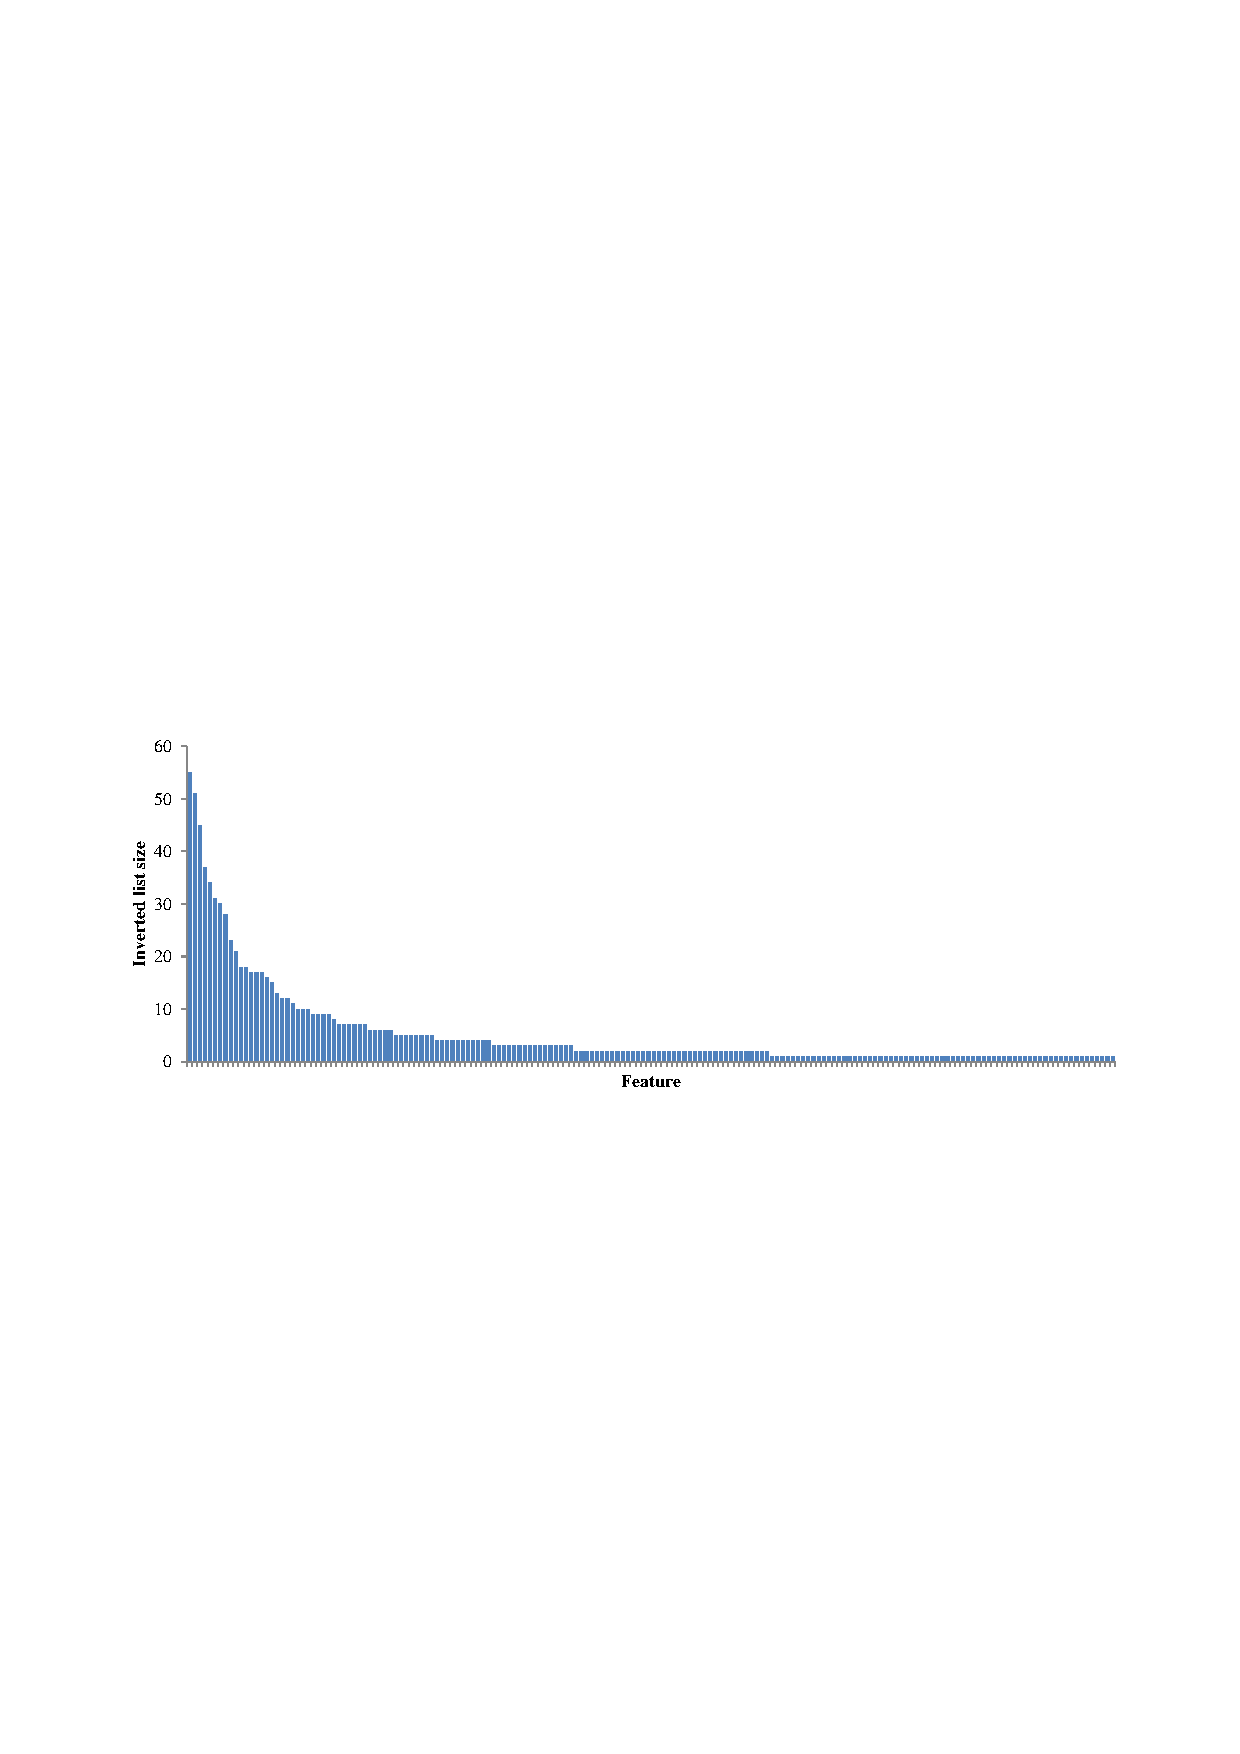
\includegraphics[width=0.4\textwidth]{graph/features.pdf}
\caption{그림 예제}
\label{fig:example1}
\end{figure}
\index{figure}


\subsection{도형 직접 그리기}

그림 \ref{fig:picture}와 같이 몇 가지 명령을 이용해서 간단한 그림을 직접 그릴 수 있다.

\begin{figure}[h!]
\centering
\setlength{\unitlength}{6pt}
\begin{picture}(40,10)
\put(20,5){\circle{6}$y$}
\put(3,2){\framebox(5,4){$x$}}
\end{picture}
\caption{간단한 도형 그리기 예제}
\label{fig:picture}
\end{figure}



\subsection{참고 문헌 관리}
각각의 참고 문헌을 bibtex 형식으로 관리하고,
다양한 형식으로 쉽게 출력할 수 있다.
bibtex에 관한 다양한 참고 문헌을 참조하기 바란다.
컴퓨터 공학 관련 분야에서는 {\em ieeetr, IEEE, unsrt, plain, abbrv}와 같은 형식이 자주 쓰인다.


\bibliographystyle{ieeetr}
\bibliography{ref}

\end{document}
